\section{Einführung}
Die Wärme ist eine Energieform. Häufig ändert sich die Temperatur $T$ eines Systems linear mit der zugeführten Wärme $\Delta Q$
\begin{equation}
	\Delta Q =C_W\Delta T =c\cdot m\cdot \Delta T\qquad,
\label{eq:waerme}
\end{equation}
wobei $C_W$ die Wärmekapazität und $c$ die spezifische Wärme ist. Dies sind materialabhängige Größen, für Wasser gilt laut\footcite{anleitung-ss2015}:
\begin{equation}
	c_{H_2 O}=\SI{4.185}{\joule\per\gram\per\kelvin}
\label{eq:cwasser}
\end{equation}

Der erste Hauptsatz der Thermodynamik verknüpft die Wärme $Q$, die einem thermodynamischen System zu- oder abgeführt wird, mit der Änderung der inneren Energie $\Delta U$ des Systems und der am bzw. vom System geleisteten mechanischen Arbeit $W$:
\begin{equation}
	Q=\Delta U - W
\label{eq:1hs}
\end{equation}
Nach Konvention hat Energie, die dem System zugeführt wird, ein positives Vorzeichen.\\

Das ideale Gas ist ein physikalisches Modell eines Gases, bei dem die Ausdehnung der Gasatome und Wechselwirkungen zwischen diesen vernachlässigt werden. Die Zustandsgleichung verknüpft den Druck $p$, das Volumen $V$, die Teilchenzahl $N$ und die Temperatur $T$:
\begin{equation}
	pV=N k_B T\qquad k_B=\SI{1.3806e-23}{J/K}
\label{eq:idgas}
\end{equation}

Durchläuft ein Stoff die Phasenübergänge fest $\rightarrow$ flüssig bzw. flüssig $\rightarrow$ fest, so wird dabei die Schmelzwärme $Q_S$ aufgenommen bzw. freigesetzt. Diese ist proportional zur Masse des Stoffes:
\begin{equation}
	Q_S=m\cdot q_S\
\label{eq:schmelz}
\end{equation}\\

Wärmekraftmaschinen wandeln Wärmeenergie in mechanische Arbeit um. Ihre Effizienz wird mit dem Wirkungsgrad angegeben (geleistete Arbeit $W$, zugeführte Wärme $Q$):
\begin{equation}
	\eta = \frac{|W|}{|Q|} \qquad \eta_c=1-\frac{T_{\text{kalt}}}{T_{\text{heiss}}}
\label{eq:wirkungsgrad}
\end{equation}
$\eta_c$ ist der maximal mögliche Wirkungsgrad (umgesetzt vom Carnot-Prozess).\\

Kältemaschinen bzw. Wärmepumpen nehmen mechanische Arbeit auf und transportieren Wärme von einem kalten Reservoir in ein warmes Reservoir. Hier wird die Effizienz durch die Leistungszahl beschrieben (aufgewandte Arbeit $W$, aus kälterem Reservoir entnommene Wärme $Q$):
\begin{equation}
	\epsilon=\frac{|Q|}{|W|}
\label{eq:leistungszahl}
\end{equation}

Der Stirling-Motor ist eine zyklisch arbeitende Wärmekraftmaschine, die thermodynamisch durch den idealisierten Stirling-Prozess beschrieben wird.
\begin{figure}[h]
  \centering
  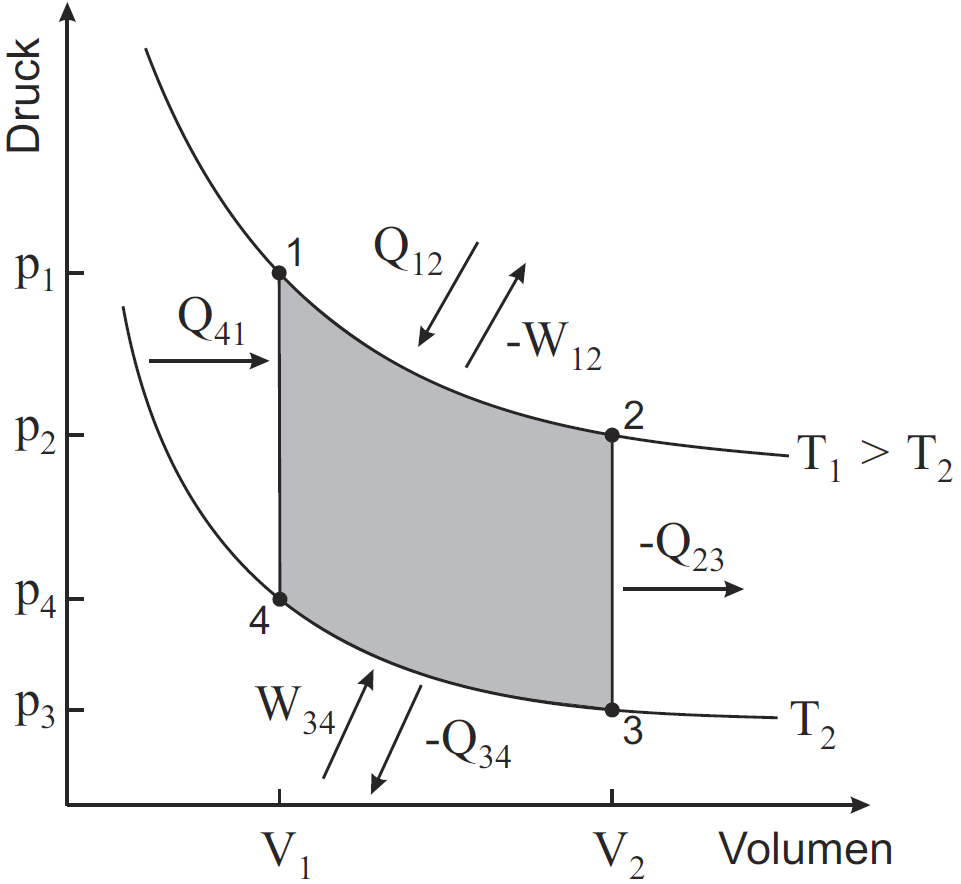
\includegraphics[width=.7\textwidth]{res/stirling_pV}
  \caption{Stirling-Kreisprozess im ($p$, $V$)-Diagramm\footcite{anleitung-ss2015}}
  \label{fig:stirling_pV}
\end{figure}
\begin{figure}[h]
  \centering
  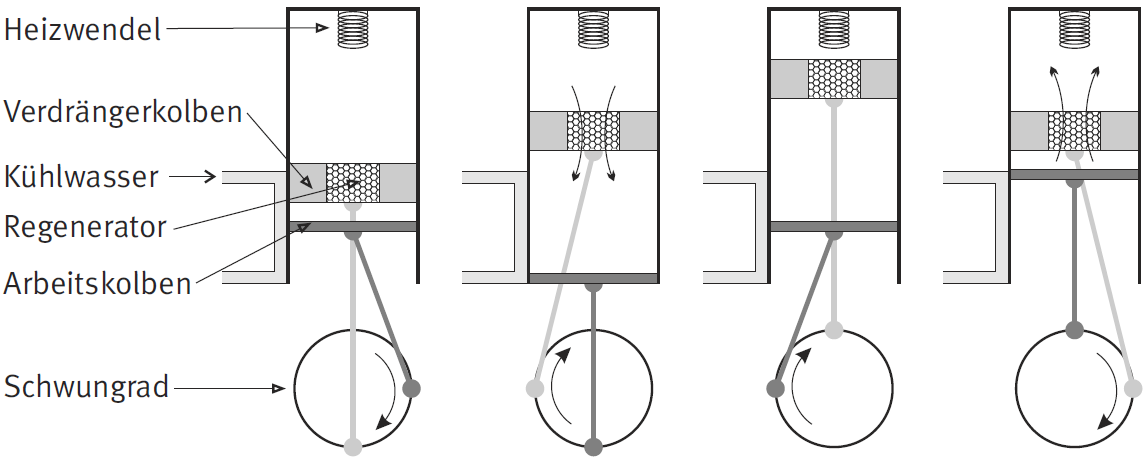
\includegraphics[width=0.9\textwidth]{res/stirling_aufbau}
  \caption{"Die Takte des Stirlingmotors. Isotherme Expansion, isochore Abkühlung, isotherme Kompression und isochore Erwärmung (von links nach rechts)"\footcite{anleitung-ss2015}}
  \label{fig:stirling_aufbau}
\end{figure}
Der Prozess durchläuft vier Teilabschnitte:

\begin{enumerate}
	\item \textbf{isotherme Expansion}: Die Luft dehnt sich bei gleich bleibender Temperatur aus, dabei wird der Arbeitskolben nach unten gedrückt und die Arbeit $-W_{12}$ am Schwungrad verrichtet. Die Wärme $Q_{12}$ wird vom Heizwendel an die Luft abgegeben. 
	\item \textbf{isochore Abkühlung}: Die Luft kühlt ab, wobei der Arbeitskolben den Tiefpunkt des Schwungrades durchläuft. Das Volumen bleibt nahezu konstant und es wird fast keine Arbeit verrichtet. Beim Hochschieben des Verdrängungskolbens wird die Luft nach unten durch den Regenerator gedrückt und dabei die Wärme $-Q_{23}$ wird an diesen abgegeben.
	\item \textbf{isotherme Kompression}: Das Schwungrad treibt den Arbeitskolben nach oben, wodurch sich das Volumen verkleinert und die Luft verdichtet wird. Dabei wird die Arbeit $W_{34}$ am System verrichtet. Die Temperatur bleibt konstant, da die Wärme $-Q_{34}$ an das Kühlwasser abgegeben wird und sich dadurch die innere Energie nicht ändert.
	\item \textbf{isochore Erwärmung}: Der Arbeitskolben durchläuft den Hochpunkt des Schwungrades, sodass das Volumen nahezu konstant bleibt und keine Arbeit verrichtet wird. Der Verdrängungskolben drückt Luft durch den Regenerator, wobei die in Schritt 2 hier gespeicherte Wärme $Q_{41}$ wieder aufgenommen wird und die Luft sich somit erwärmt.
\end{enumerate}

Wird der Heizwendel entfernt und das Schwungrad mit einem Motor angetrieben, so wird der Prozess umgekehrt und der Stirling-Motor arbeitet stattdessen als Kältemaschine (bzw. Wärmepumpe bei anderer Drehrichtung). Pro Umlauf wird die Wärme $Q_2$ dem Zylinderkopf entzogen und die Wärme $-Q_1$ dem Kühlwasser zugeführt. Durch Kolbenreibung wird außerdem eine Reibungsarbeit $W_R$ aufgewandt und in thermische Energie umgewandelt. Für die Arbeit $W$, die der Motor pro Umlauf am Schwungrad leisten muss, gilt also:
\begin{equation}
	W=Q_1-Q_2+W_R
\label{eq:reibungsarbeit}
\end{equation}

\section{Versuch}
Am Praktikumstag stand ein Stirling-Motor analog zu \cref{fig:stirling_aufbau} zur Verfügung. Das Kühlwasser wurde in einem Kreislauf in einen großen Wasserbehälter gepumpt. Über einen Winkelmaßgerät wurde die Stellung des Arbeitskolbens digitalisiert, außerdem wurde der Druck im Zylinder gemessen.
\subsection{Betrieb als Wärmepumpe bzw. Kältemaschine}
\subsubsection{Bestimmung der Reibungsverluste}
Zunächst wurde der Reibungsverlust durch Kolbenreibung anhand der Erwärmung des Kühlwassers bestimmt.
Der Volumendurchsatz des Kühlwassers wurde mit Stoppuhr und Messkolben gemessen: In $t=\SI{21.13(20)}{s}$ flossen $V=\SI{82(1)}{ml}$ Wasser, was einem Durchsatz von $D=\SI{3.88(6)}{ml/s}$ entspricht. Vor dem Versuch betrug die Temperatur am Kühlwasserabfluss des Zylinders $T_0=\SI{22.3(1)}{\degreeCelsius}$. Der Motor wurde bei offenem Zylinderkopf mit einer Frequenz $f=\SI{3.05(2)}{Hz}$ (bestimmt durch FFT des Winkelsignals mit LabVIEW) betrieben, bis sich die Temperatur am Kühlwasserabfluss nicht mehr geändert hat. Es stellte sich eine Gleichgewichtstemperatur $T_1=\SI{22.7(1)}{\degreeCelsius}$ ein. Die pro Umlauf an das Kühlwasser abgegebene Wärme (d.h. die Kolbenreibungsarbeit pro Umlauf) beträgt dann
\begin{align}
	W_R&=\frac{D}{f}\cdot \rho_{H_2O}\cdot c_{H_2O}(T_1-T_0) \\
	&=\frac{\SI{3.88(6)}{ml/s}}{\SI{3.05(2)}{Hz}}\cdot \SI{1}{\g\per\cubic\cm}\cdot \SI{4.185}{\joule\per\gram\per\kelvin}\cdot \SI{.4(2)}{K} \\
	&=\SI{2.13(107)}{J}
\label{eq:reibungswaerme}
\end{align}
\subsubsection{Bestimmung der Kühlleistung}
In ein Reagenzglas wurden mit einer Pipette \SI{1.00(2)}{ml} destilliertes Wasser gefüllt und dieses auf den Zylinderkopf aufgesetzt. Der Motor wurde auf dieselbe Drehzahl wie in Teil 1 eingestellt und die Temperatur des Wassers wurde digital aufgenommen.
\begin{figure}[h!]
\centering
\begin{tikzpicture}
  \begin{axis}[
    width=15 cm,
    height=9 cm,
    xmin=0, xmax=1165,
    ymin=-26, ymax=23,
    xlabel={Zeit $t$ [\si{s}]},
    ylabel={Temperatur $T$ [\si{\degreeCelsius}]},
    domain=0:220,
    legend entries={Temperatur des Wassers im RG, $\SI{-0.1482}{\degreeCelsius\per\s}\cdot x+\SI{22.9219}{\degreeCelsius}$},
    legend pos=north east
  ]
  \addplot+ plot [only marks,mark=x, error bars/.cd, x dir=both, x fixed=0.2, y dir=both, y fixed=0.1]  table[skip first n=2, my filter=every 50 except 1113 and 1137 there 2, filter discard warning=false, unbounded coords=discard] {res/Nr2_Temp_Zeit.txt};
	\addplot+ plot [mark=none]  {-0.1482*x+22.9219};
	\draw ({axis cs:223,0}|-current axis.south) -- ({axis cs:223,0}|-current axis.north);
	\draw ({axis cs:385,0}|-current axis.south) -- ({axis cs:385,0}|-current axis.north);
  \end{axis}
\end{tikzpicture}
\caption{Temperatur von \SI{1}{ml} Wasser im Reagenzglas am Zylinderkopf bei Betrieb des Stirling-Motors als Kältemaschine}
\label{fig:kaeltemaschine}
\end{figure}

Zu sehen ist, dass die Temperatur wie erwartet abfällt. Nach ca. \SI{220}{s} erreicht sie vorerst einen Tiefpunkt bei \SI{-5.5}{\degreeCelsius}. Bis zu diesem Zeitpunkt wurde während des Versuches beobachtet, dass das Wasser noch nicht gefroren war. Bei $t_1=\SI{223(1)}{s}$ bildete sich Frost an der Reagenzglaswand und die Temperatur stieg schnell auf \SI{0.4}{\degreeCelsius} an, wo sie bis $t_2=\SI{385(1)}{s}$ konstant blieb (vgl vertikale Linien in \cref{fig:kaeltemaschine}). Ab da folgte ein monotoner Abfall auf \SI{-25.4}{\degreeCelsius}.

Um die Steigung der Abkühlkurve zu bestimmen, wurde mit gnuplot nach dem \emph{least-squares-}Verfahren der Bereich zwischen \SI{13.2}{s} und {150}{s} gegen die Funktion $f(x)=a\cdot x+b$ gefittet (rote Linie in \cref{fig:kaeltemaschine}). Dieser Bereich wurde so gewählt, da in den ersten \SI{13}{s} noch keine Temperaturänderung gemessen wurde (Anlaufphase des Motors, Reagenzglas muss sich erst abkühlen) und da bei größerem Abstand zur Zimmertemperatur der Wärmeverlust durch Wärmeleitung des Zylinderglases zu groß wird.
Die Steigung beträgt $a=\SI{-0.1482(5)}{\degreeCelsius\per\s}$, was einer Kühlleistung von 
\begin{align}
	P_K&=|a|\cdot V\cdot\rho_{H_2O}\cdot c_{H_2O}\\
	&=\SI{-0.1482(5)}{\degreeCelsius\per\s}\cdot \SI{1}{ml}\cdot\SI{1}{\g\per\cubic\cm}\cdot \SI{4.185}{\joule\per\gram\per\kelvin} \\
	&=\SI{0.6202(21)}{J/s}
\label{eq:kuehlleistung}
\end{align}
bzw. einer dem Wasser im RG entzogenen Wärme pro Umlauf von 
\begin{equation}
	Q_2=P_K/f=\frac{\SI{0.6202(21)}{J/s}}{\SI{3.05(2)}{Hz}}=\SI{0.2033(15)}{J}
\label{eq:kuehlleistung}
\end{equation}
entspricht.

Das Plateau von $t_1=\SI{223(1)}{s}$ bis $t_2=\SI{385(1)}{s}$ wird als der Zeitraum interpretiert, währenddessen die von der Kältemaschine entzogene Wärme vollständig von der frei werdenden Schmelzwärme $Q_S$ des Wassers kompensiert wird, sodass sich die Temperatur nicht ändert. Die Schmelzwärme beträgt also 
\begin{equation}
	Q_S=P\cdot (t_2-t_1)=\SI{0.6202(21)}{J/s}\cdot\SI{162(2)}{s}=\SI{100.47(128)}{J}\qquad.
\label{eq:schmelzberechnet}
\end{equation}

Die Temperaturen des abfließenden Kühlwassers sowie des Wasserreservoirs wurden vor und nach der Aufnahme der Abkühlkurve mit dem Thermometer gemessen:
\begin{table}[H]
\centering
\begin{tabular}{c | c c}
		& vorher & nachher  \\ \midrule
		abfl. Kühlwasser & $T_0=\SI{22.3(1)}{\degreeCelsius}$ & $T_1=\SI{23.9(1)}{\degreeCelsius}$ \\
		Wasserreservoir & \SI{22.0(1)}{\degreeCelsius} & \SI{22.8(1)}{\degreeCelsius}
\end{tabular}
\caption{Wassertemperaturen vor und nach Betrieb der Kältemaschine}
\label{tab:wassertemps}
\end{table}

Die pro Umlauf an das Kühlwasser abgegebene Wärme wird analog zu \cref{eq:reibungswaerme} ermittelt:
\begin{align}
	Q_1&=\frac{D}{f}\cdot \rho_{H_2O}\cdot c_{H_2O}(T_1-T_0) \\
	&=\frac{\SI{3.88(6)}{ml/s}}{\SI{3.05(2)}{Hz}}\cdot \SI{1}{\g\per\cubic\cm}\cdot \SI{4.185}{\joule\per\gram\per\kelvin}\cdot \SI{1.6(2)}{K} \\
	&=\SI{8.52(107)}{J}
\label{eq:q2}
\end{align}

Die Leistungszahl ergibt sich mit der in Teil 1 berechneten Reibungsarbeit pro Umlauf zu
\begin{align}
	\epsilon&=\frac{Q_2}{W}=\frac{Q_2}{Q_1-Q_2+W_R}\\
	&=\frac{\SI{0.2033(15)}{J}}{\SI{8.52(107)}{J}-\SI{0.2033(15)}{J}+\SI{2.13(107)}{J}}\\
	&=\SI{1.95(39)}{\percent}\qquad.
\label{eq:schmelzberechnet}
\end{align}

\subsubsection{Bestimmung der Heizleistung}
Nun wird der Motor bei gleich bleibender Drehzahl in umgekehrter Umlaufrichtung betrieben und die Aufwärmkurve des Wassers aufgenommen.